汽车电子架构变得越发复杂,包括越来越多的传感器、控制器和接口,对通信带宽、链路和速率有了更高的要求。
以太网通信相较于传统的车载通信方式,如 CAN、LIN 等,具有高通信速率的显著优势。
本章将基于 AutoSar 软件架构及 Vector 工具链完成相关模块的配置,以实现基本的以太网通信。

\section{物理层}

\section{链路层}

\subsection{链路聚合}
链路聚合\cite{Link_Aggregation}(英语:Link Aggregation)是一个计算机网络术语,指将多个物理端口汇聚在一起,形成一个逻辑端口,
以实现出/入流量吞吐量在各成员端口的负荷分担,交换机根据用户配置的端口负荷分担策略决定网络封包从哪个成员端口发送到对端的交换机。
当交换机检测到其中一个成员端口的链路发生故障时,就停止在此端口上发送封包,并根据负荷分担策略在剩下的链路中重新计算报文的发送端口,
故障端口恢复后再次担任收发端口。链路聚合在增加链路带宽、实现链路传输弹性和工程冗余等方面是一项很重要的技术。

\subsubsection{链路聚合原理}

\begin{itemize}
    \item 把聚合后得到的逻辑链路称为聚合链路,把聚合链路中的每一条物理链路称为成员链路。
    \item 把聚合后得到的逻辑端口称为聚合端口,把聚合端口中的每一个物理端口称为成员端口。
    \item 聚合链路也被称为Eth-Trunk链路,聚合端口也被称为Eth-Trunk端口。
\end{itemize}

\begin{figure}[ht]
    \centering
    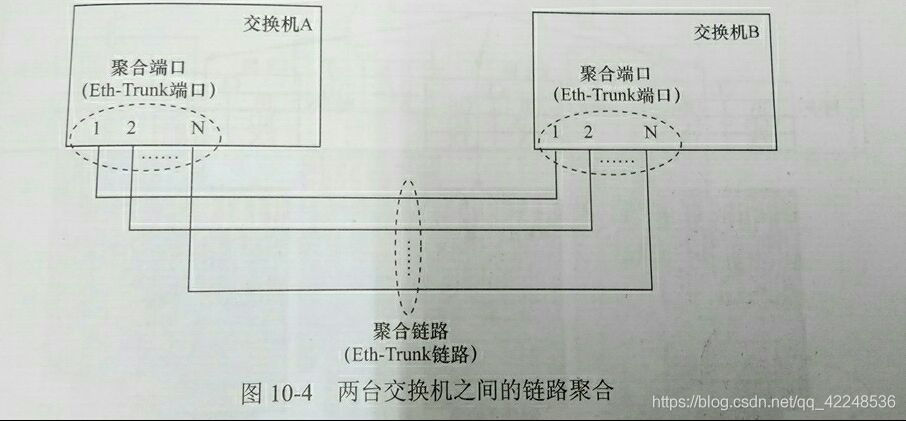
\includegraphics[scale=0.5]{pic/20190414170741211.jpg}
    \caption{交换机链路聚合}
    \label{fig:switch_link_aggre}
\end{figure}

交换机A是怎样通过自己的 Eth-Trunk 端口向交换机 B 的 Eth-Trunk 端口发送帧的?

\begin{enumerate}
    \item 来自交换机A的其他端口的帧进入到Eth-Trunk端口的帧发送队列;
    \item Eth-Trunk端口的帧分发器(FD)将这些帧按照某种算法依次发给成员端口。FD的分发顺序是:先将Frame A发给某个成员端口,再将Frame b发给某个成员端口,依次类推;
    \item 每个成员端口按照常规方法将来自FD的帧发送到自己的物理链路上。如图\ref{fig:switch_link_aggre_transmit}所示。
\end{enumerate}

假若FD能够非常均匀的将帧分发给不同的成员端口,则 Eth-Trunk 端口的带宽就等于各成员端口的带宽之和,而 Eth-Trunk 链路的带宽就等于各成员链路的带宽之和。

但是,FD 对帧的分发并不是非常均匀的,所以 \textcolor{red}{\textbf{Eth-Trunk 链路实际上能够提供的最大的链路带宽一般会小于各成员链路带宽的总和}}。

\begin{figure}[ht]
    \centering
    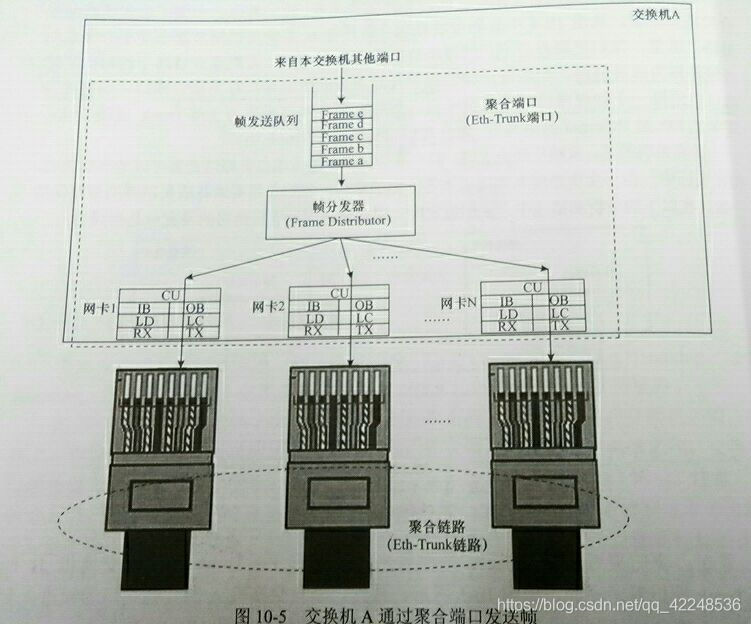
\includegraphics[scale=0.5]{pic/20190414171718383.jpg}
    \caption{链路聚合数据发送}
    \label{fig:switch_link_aggre_transmit}
\end{figure}

交换机B是怎样从自己的Eth-Trunk端口接收到来自交换机A的Eth-Trunk端口发送过来的帧?

\begin{enumerate}
    \item 每个成员端口会按照常规方式接收来自物理链路上的帧,将接收到的帧送到Eth-Trunk端口的帧收集器(FC);
    \item 当帧“完全进入”(指:帧的末尾也进入到FC中)到FC中后,FC会将它送至Eth-Trunk端口的帧接收队列中;
    \item 最先完全进入FC的帧是Frame a,其次是Frame b,等等类推。
    \item Eth-Trunk端口的帧接收队列中的帧会被依次的送往交换机B 的其他端口。
\end{enumerate}

\begin{remark}
    链路聚合的基本原理就是“流量分担”原理:多条成员链路共同分担了聚合链路的总流量。如果聚合链路中的某一条成员链路发生故障而中断了,那么聚合链路的总流量会继续呗其他的成员链路来分担(本该由故障链路所分担的流量将会被FD转移到其他的成员链路)。
\end{remark}

\subsubsection{链路聚合乱序问题}
所谓的乱序现象就是指:交换机B的帧接收队列中帧的排序不同于其在交换机A的帧发送队列中的顺序。乱序现象分为两种:有害乱序、无害乱序。
有害的乱序:会多少的对网络应用程序有所影响。无害的乱序:交换机B的帧接收队列中发生的乱序现象是一种无害的乱序。

聚合链路在工作的过程中,由于帧的长度有所不同,则帧的传输时间就会有所不同,有长有短的时间,同时不同的帧所经过的成员链路也可能不同,
所有在一般情况下总是会出现乱序现象。虽然无法避免乱序现象的发生,但是可以尽可能的避免有害乱序现象的发生。

避免有害乱序现象的关键是:\textbf{聚合端口的FD是怎样将帧分发给不同的成员端口的}。

\subsubsection{Conversation 概念}
一个Conversation是指由若干个帧组成的一个集合,该集合中的不同的帧在接收端的聚合端口的帧的接收队列中的先后顺序必须与它们在发送端的聚合端口的帧的发送队列中的先后顺序保持一致。如果保持了一致,则一定不会发生有害乱序现象;若没有保持一致,则一定会发生有害乱序现象。

\begin{remark}
    不同的Conversation之间的交集必须是一个空集,即同一个帧,不能既属于这个Conversation,又属于另外一个Conversation;一个帧不能不属于任何Conversation。
\end{remark}


聚合端口需要遵从的分发原则:
\begin{enumerate}
    \item 同一个Conversation中的帧,必须被分发给同一条成员端口(可避免有害乱序现象);
    \item 不同Conversation中的帧,可以被分发给同一个成员链路,也可以被分发给不同的成员链路(可实现流量分担);
\end{enumerate}

图\ref{fig:switch_link_aggre_conversation_transmit}中:交换机A的聚合端口首先会对帧的发送队列中的帧进行Conversation划分,
划分的方法是:把具有相同目的MAC地址的帧分进同一个Conversation,而且要保证同一个Conversation中的帧都具有相同的目的MAC地址。
\begin{figure}[ht]
    \centering
    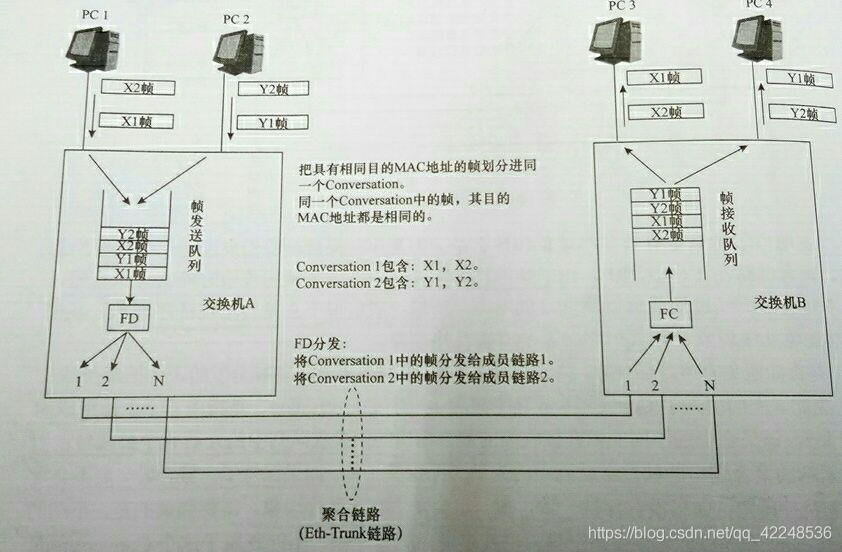
\includegraphics[scale=0.5]{pic/20190414180436629.jpg}
    \caption{链路聚合数据Conversation发送}
    \label{fig:switch_link_aggre_conversation_transmit}
\end{figure}

在实际的链路聚合实现中,聚合链路的FD需要根据HASA算法来定义出恰当的Conversation,然后再对不同的Conversation进行分发。(该图中的目的MAC地址被选择成用来定义Conversation的参考量)。

在实际的网络环境中,聚合链路的两端的设备属性(如:交换机和路由器,等等)以及上层应用的属性,都需要称为确定Conversation的参考量的考虑因素,最终可能参考的是目的MAC地址或者源MAC地址,等等。

\subsection{ENET 中断分析}

ENET 由中断触发到上层数据接收并处理的过程见下图。

\begin{figure}[ht]
    \centering
    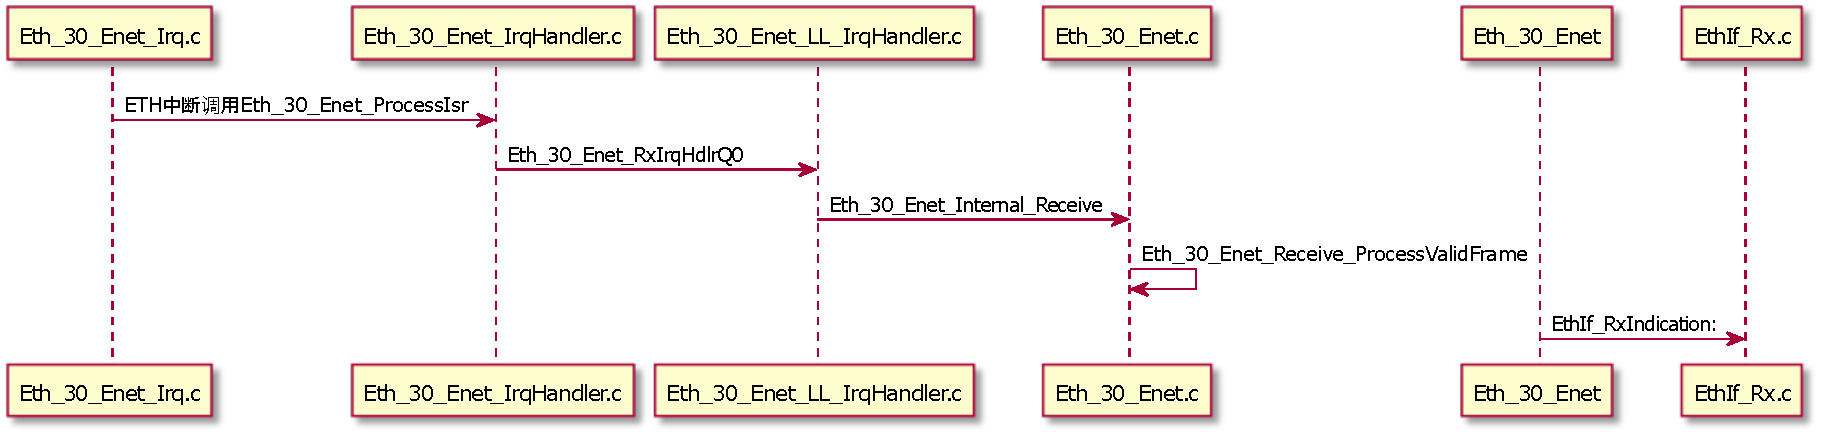
\includegraphics[scale=0.5]{pic/eth_isr.pdf}
    \caption{ENET 中断代码调用}
    \label{fig:enet_isr}
\end{figure}

其中 \lstinline{Eth_30_Enet_Irq.c} 中包含 \lstinline{OS} 中配置的 \lstinline{ENET} 中断处理函数:

\begin{lstlisting}[language=C]
ISR( EthIsr_EthernetCnt_MCU_Ctrl_ad7672f0_EthInterruptServiceRoutine_Q0Rx );
ISR( EthIsr_EthernetCnt_MCU_Ctrl_ad7672f0_EthInterruptServiceRoutine_Q0Tx );
\end{lstlisting}

后续通过 \lstinline{Eth_30_Enet_Internal_Receive} 处理接收到的数据帧,其中由 \lstinline{Eth_30_Enet_Receive_ProcessValidFrame} 验证数据帧后,由 \lstinline{EthIf_RxIndication} 传至上层模块。

\section{网络层}
\subsection{组播}
\subsubsection{组播地址}

组播报文的目的地址使用D类IP地址, D类地址不能出现在IP报文的源IP地址字段。

单播数据传输过程中,一个数据包传输的路径是从源地址路由到目的地址,利用“逐跳”的原理在IP网络中传输。

然而在ip组播环中,数据包的目的地址不是一个,而是一组,形成组地址。

所有的信息接收者都加入到一个组内,并且一旦加入之后,流向组地址的数据立即开始向接收者传输,组中的所有成员都能接收到数据包。
组播组中的成员是动态的,主机可以在任何时刻加入和离开组播组。

\subsubsection{范围}

\begin{itemize}
    \item 224.0.0.0~224.0.0.255为预留的组播地址(永久组地址),地址224.0.0.0保留不做分配,其它地址供路由协议使用;
    \item 224.0.1.0~224.0.1.255是公用组播地址,可以用于Internet;
    \item 224.0.2.0~238.255.255.255为用户可用的组播地址(临时组地址),全网范围内有效;
    \item 239.0.0.0~239.255.255.255为 \textbf{本地} 管理组播地址,仅在特定的本地范围内有效。

\end{itemize}

\subsubsection{组播IP地址和MAC地址转换}

组播MAC地址有IP地址映射转换而成,过程如下图所示:

\begin{figure}[ht]
    \centering
    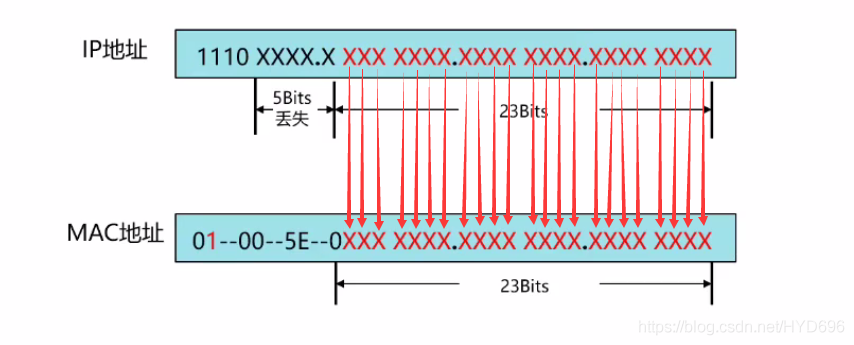
\includegraphics[scale=0.7]{pic/multicast-01.png}
    \caption{multicast ip addr to mac}
    \label{fig:multicast_ip_addr_to_mac}
\end{figure}


过程如下:

\begin{enumerate}
    \item 加上MAC地址固定前缀(24bit)为:01-00-5E;
    \item 后面24bit由IP地址的后23bit构成;
    \item 第25 bit位固定为0;
\end{enumerate}

\subsubsection{举例}

以Someip SD服务组播地址为例,组播IP地址为 \textbf{239.127.3.1}。

\begin{itemize}
    \item 二进制: \textbf{1110 1111 0111 1111 0000 0011 0000 0001}
    \item 固定前缀: \textbf{01-00-5E- + 0b}
    \item 转换结果: \textbf{01-00-5e-7f-03-01}
\end{itemize}

\subsubsection{代码实现}

协议栈中由TCPIP模块分配多播IP地址到设置 \lstinline{ENET multicast mac filter ENETn_GAUR/GALR}寄存器的过程如下图所示:

\begin{figure}[h]
    \centering
    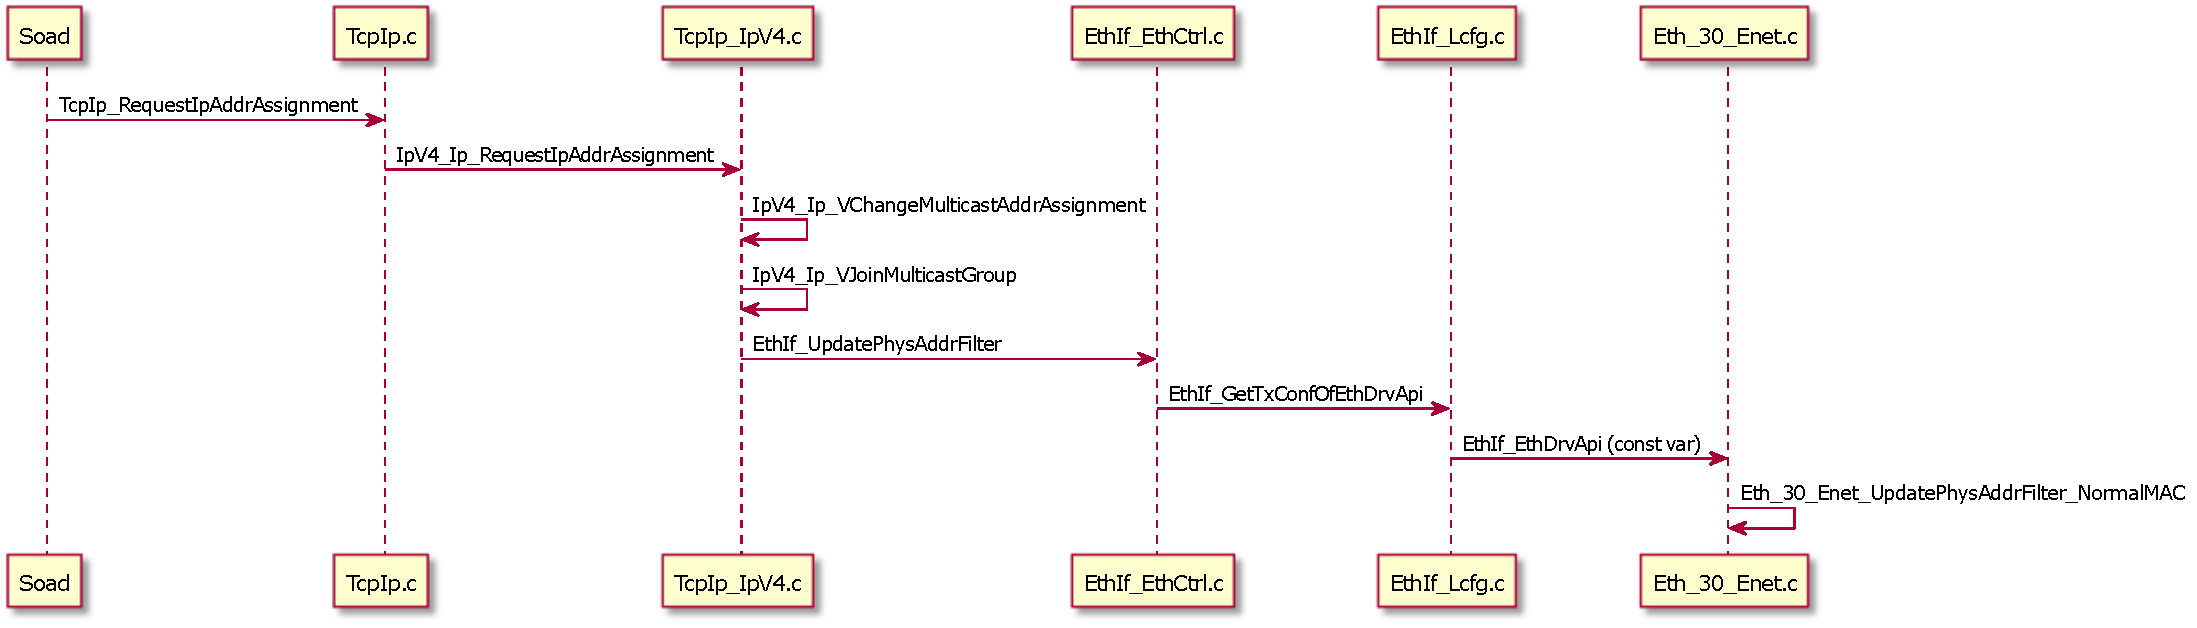
\includegraphics[scale=0.5]{pic/eth_multicast_mac_code.pdf}
    \caption{eth multicast mac code}
    \label{fig:eth_multicast_mac_code}
\end{figure}